\ifdefined\included
\else
\documentclass[a4paper,11pt,twoside]{StyleThese}
\usepackage{amsmath,amssymb, amsthm}             % AMS Math
\usepackage[T1]{fontenc}
\usepackage[utf8x]{inputenc}
\usepackage{babel}
\usepackage{datetime}

\usepackage{silence}

\WarningFilter{minitoc(hints)}{W0023}
\WarningFilter{minitoc(hints)}{W0028}
\WarningFilter{minitoc(hints)}{W0030}

\usepackage{lmodern}
\usepackage{tabularx}
%\usepackage{tabular}
\usepackage{multirow}
\usepackage{xspace}

\usepackage{subfig}
\usepackage[inline]{enumitem}

\usepackage{hhline}
\usepackage[left=1.5in,right=1.3in,top=1.1in,bottom=1.1in,includefoot,includehead,headheight=13.6pt]{geometry}
\renewcommand{\baselinestretch}{1.05}

% Table of contents for each chapter

\usepackage[nottoc, notlof, notlot]{tocbibind}
\usepackage{minitoc}
\setcounter{minitocdepth}{2}
\mtcindent=15pt
% Use \minitoc where to put a table of contents

\usepackage{aecompl}

% Glossary / list of abbreviations

\usepackage[intoc]{nomencl}
\iftoggle{ThesisInEnglish}{%
\renewcommand{\nomname}{Glossary}
}{ %
\renewcommand{\nomname}{Liste des Abréviations}
}

\usepackage{etoolbox}
\renewcommand\nomgroup[1]{%
  \item[\bfseries
  \ifstrequal{#1}{A}{Number Sets}{%
  \ifstrequal{#1}{G}{Agents Beliefs and Action Models}{%
  \ifstrequal{#1}{N}{Navigation}{%
  \ifstrequal{#1}{O}{Ontology}{%
  \ifstrequal{#1}{R}{Referring Expression Generation}{%
  \ifstrequal{#1}{Z}{Controllable and Uncontrollable Agents Task Planning}{}}}}}}%
]}

\makenomenclature



% My pdf code

\usepackage{ifpdf}

\ifpdf
  \usepackage[pdftex]{graphicx}
  \DeclareGraphicsExtensions{.jpg}
  \usepackage[pagebackref,hyperindex=true]{hyperref}
  \usepackage{tikz}
  \usetikzlibrary{arrows,shapes,calc}
\else
  \usepackage{graphicx}
  \DeclareGraphicsExtensions{.ps,.eps}
  \usepackage[dvipdfm,pagebackref,hyperindex=true]{hyperref}
\fi

\graphicspath{{.}{images/}}

%% nicer backref links. NOTE: The flag ThesisInEnglish is used to define the
% language in the back references. Read more about it in These.tex

\iftoggle{ThesisInEnglish}{%
\renewcommand*{\backref}[1]{}
\renewcommand*{\backrefalt}[4]{%
\ifcase #1 %
(Not cited.)%
\or
(Cited in page~#2.)%
\else
(Cited in pages~#2.)%
\fi}
\renewcommand*{\backrefsep}{, }
\renewcommand*{\backreftwosep}{ and~}
\renewcommand*{\backreflastsep}{ and~}
}{%
\renewcommand*{\backref}[1]{}
\renewcommand*{\backrefalt}[4]{%
\ifcase #1 %
(Non cité.)%
\or
(Cité en page~#2.)%
\else
(Cité en pages~#2.)%
\fi}
\renewcommand*{\backrefsep}{, }
\renewcommand*{\backreftwosep}{ et~}
\renewcommand*{\backreflastsep}{ et~}
}

% Links in pdf
\usepackage{color}
\definecolor{linkcol}{rgb}{0,0,0.4} 
\definecolor{citecol}{rgb}{0.5,0,0} 
\definecolor{linkcol}{rgb}{0,0,0} 
\definecolor{citecol}{rgb}{0,0,0}
% Change this to change the informations included in the pdf file

\hypersetup
{
bookmarksopen=true,
pdftitle="Endowing the robot with the abilities to control and evaluate its contribution to a human-robot joint action",
pdfauthor="Amandine MAYIMA", %auteur du document
pdfsubject="Thèse", %sujet du document
%pdftoolbar=false, %barre d'outils non visible
pdfmenubar=true, %barre de menu visible
pdfhighlight=/O, %effet d'un clic sur un lien hypertexte
colorlinks=true, %couleurs sur les liens hypertextes
pdfpagemode=None, %aucun mode de page
pdfpagelayout=SinglePage, %ouverture en simple page
pdffitwindow=true, %pages ouvertes entierement dans toute la fenetre
linkcolor=linkcol, %couleur des liens hypertextes internes
citecolor=citecol, %couleur des liens pour les citations
urlcolor=linkcol %couleur des liens pour les url
}

% definitions.
% -------------------

\setcounter{secnumdepth}{3}
\setcounter{tocdepth}{2}

% Some useful commands and shortcut for maths:  partial derivative and stuff

\newcommand{\pd}[2]{\frac{\partial #1}{\partial #2}}
\def\abs{\operatorname{abs}}
\def\argmax{\operatornamewithlimits{arg\,max}}
\def\argmin{\operatornamewithlimits{arg\,min}}
\def\diag{\operatorname{Diag}}
\newcommand{\eqRef}[1]{(\ref{#1})}

\usepackage{rotating}                    % Sideways of figures & tables
%\usepackage{bibunits}
%\usepackage[sectionbib]{chapterbib}          % Cross-reference package (Natural BiB)
%\usepackage{natbib}                  % Put References at the end of each chapter
                                         % Do not put 'sectionbib' option here.
                                         % Sectionbib option in 'natbib' will do.
\usepackage{fancyhdr}                    % Fancy Header and Footer

% \usepackage{txfonts}                     % Public Times New Roman text & math font
  
%%% Fancy Header %%%%%%%%%%%%%%%%%%%%%%%%%%%%%%%%%%%%%%%%%%%%%%%%%%%%%%%%%%%%%%%%%%
% Fancy Header Style Options

\pagestyle{fancy}                       % Sets fancy header and footer
\fancyfoot{}                            % Delete current footer settings

%\renewcommand{\chaptermark}[1]{         % Lower Case Chapter marker style
%  \markboth{\chaptername\ \thechapter.\ #1}}{}} %

%\renewcommand{\sectionmark}[1]{         % Lower case Section marker style
%  \markright{\thesection.\ #1}}         %

\fancyhead[LE,RO]{\bfseries\thepage}    % Page number (boldface) in left on even
% pages and right on odd pages
\fancyhead[RE]{\bfseries\nouppercase{\leftmark}}      % Chapter in the right on even pages
\fancyhead[LO]{\bfseries\nouppercase{\rightmark}}     % Section in the left on odd pages

\let\headruleORIG\headrule
\renewcommand{\headrule}{\color{black} \headruleORIG}
\renewcommand{\headrulewidth}{1.0pt}
\usepackage{colortbl}
\arrayrulecolor{black}

\fancypagestyle{plain}{
  \fancyhead{}
  \fancyfoot{}
  \renewcommand{\headrulewidth}{0pt}
}

%\usepackage{MyAlgorithm}
%\usepackage[noend]{MyAlgorithmic}
\usepackage{algorithm}
\usepackage[noend]{algpseudocode}
\usepackage{comment}
\usepackage[ED=MITT-InfoTel, Ets=INSA]{tlsflyleaf}
%%% Clear Header %%%%%%%%%%%%%%%%%%%%%%%%%%%%%%%%%%%%%%%%%%%%%%%%%%%%%%%%%%%%%%%%%%
% Clear Header Style on the Last Empty Odd pages
\makeatletter

\def\cleardoublepage{\clearpage\if@twoside \ifodd\c@page\else%
  \hbox{}%
  \thispagestyle{empty}%              % Empty header styles
  \newpage%
  \if@twocolumn\hbox{}\newpage\fi\fi\fi}

\newcommand*{\algrule}[1][\algorithmicindent]{%
	\makebox[#1][l]{%
		\hspace*{.2em}% <------------- This is where the rule starts from
		\vrule height .75\baselineskip depth .25\baselineskip
	}
}

%%% to have lines in algorithm, from stackexchange
\newcount\ALG@printindent@tempcnta
\def\ALG@printindent{%
	\ifnum \theALG@nested>0% is there anything to print
	\ifx\ALG@text\ALG@x@notext% is this an end group without any text?
	% do nothing
	\else
	\unskip
	% draw a rule for each indent level
	\ALG@printindent@tempcnta=1
	\loop
	\algrule[\csname ALG@ind@\the\ALG@printindent@tempcnta\endcsname]%
	\advance \ALG@printindent@tempcnta 1
	\ifnum \ALG@printindent@tempcnta<\numexpr\theALG@nested+1\relax
	\repeat
	\fi
	\fi
}
% the following line injects our new indent handling code in place of the default spacing
\patchcmd{\ALG@doentity}{\noindent\hskip\ALG@tlm}{\ALG@printindent}{}{\errmessage{failed to patch}}
\patchcmd{\ALG@doentity}{\item[]\nointerlineskip}{}{}{} % no spurious vertical space
% end vertical rule patch for algorithmicx

\makeatother
 
%%%%%%%%%%%%%%%%%%%%%%%%%%%%%%%%%%%%%%%%%%%%%%%%%%%%%%%%%%%%%%%%%%%%%%%%%%%%%%% 
% Prints your review date and 'Draft Version' (From Josullvn, CS, CMU)
\newcommand{\reviewtimetoday}[2]{\special{!userdict begin
    /bop-hook{gsave 20 710 translate 45 rotate 0.8 setgray
      /Times-Roman findfont 12 scalefont setfont 0 0   moveto (#1) show
      0 -12 moveto (#2) show grestore}def end}}
% You can turn on or off this option.
% \reviewtimetoday{\today}{Draft Version}
%%%%%%%%%%%%%%%%%%%%%%%%%%%%%%%%%%%%%%%%%%%%%%%%%%%%%%%%%%%%%%%%%%%%%%%%%%%%%%% 

\newenvironment{maxime}[1]
{
\vspace*{0cm}
\hfill
\begin{minipage}{0.5\textwidth}%
%\rule[0.5ex]{\textwidth}{0.1mm}\\%
\hrulefill $\:$ {\bf #1}\\
%\vspace*{-0.25cm}
\it 
}%
{%

\hrulefill
\vspace*{0.5cm}%
\end{minipage}
}

\let\minitocORIG\minitoc
\renewcommand{\minitoc}{\minitocORIG \vspace{1.5em}}

\usepackage{multirow}
%\usepackage{slashbox}

\newenvironment{bulletList}%
{ \begin{list}%
	{\tiny$\bullet$}%
	{\setlength{\labelwidth}{25pt}%
	 \setlength{\leftmargin}{30pt}%
	 \setlength{\itemsep}{-0.5em}}}%
{ \end{list} }

\newenvironment{inlineEnumerate}
{\begin{enumerate*} [label={(\arabic*)}] }
{\end{enumerate*}}

\theoremstyle{definition}
\newtheorem{definition}{Definition}
\renewcommand{\epsilon}{\varepsilon}

% centered page environment

\newenvironment{vcenterpage}
{\newpage\vspace*{\fill}\thispagestyle{empty}\renewcommand{\headrulewidth}{0pt}}
{\vspace*{\fill}}

\newenvironment{asl}{\ttfamily\begin{tabbing}~~~\=$\leftarrow$ \= ~~~ \=
		\kill}{\end{tabbing}}

\usepackage{tablefootnote}

\theoremstyle{plain}
\newtheorem{constraint}{Constraint}[section]

\algnewcommand\algorithmicforeach{\textbf{for each}}
\algnewcommand\algorithmicin{\textbf{in}}
\algdef{S}[FOR]{ForEach}[2]{\algorithmicforeach\ #1\ \algorithmicin\ #2\ \algorithmicdo}

\algnewcommand\algorithmicforkxor{\textbf{do fork-join-xor}}
\algnewcommand\algorithmicendforkxor{\textbf{end fork-join-xor}}
\algdef{SE}{ForkXor}{EndForkXor}{\algorithmicforkxor}{\algorithmicendforkxor}


\usepackage{listings}
\lstset{
	frame=single,
	captionpos=b,
	breaklines=true,
	basicstyle=\ttfamily,
	numberstyle=\color{black},
	tabsize=2,
	mathescape=true,
	literate=%
		{â}{{\^a}}1
}

\lstdefinestyle{inline}{
	frame=none,
	aboveskip=\smallskipamount,
	belowskip=\smallskipamount,
}

\lstdefinestyle{OwlTurtle}{
	language=C,
	tabsize=4,
	basicstyle=\scriptsize\ttfamily,
	keywordstyle=\bfseries\color{darkgray},
	morekeywords={rdf:type, rdfs:domain, rdfs:subPropertyOf, rdfs:range, :hasSubtask, :DecompositionUsedBy, rdfs:subClassOf, :hasDecomposition, owl:inverseOf, htn_actions:hasEffect, rdfs:label},
	alsoletter=:
}

\lstdefinestyle{aslDef}{
	frame=none,
%	breaklines=false,
	%xleftmargin=.1\textwidth, xrightmargin=.1\textwidth
}

\fancypagestyle{example}{%
	\fancyhead[LE]{\bfseries\thepage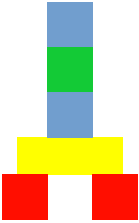
\includegraphics[scale=0.20]{figures/chapter2/task_goal.pdf}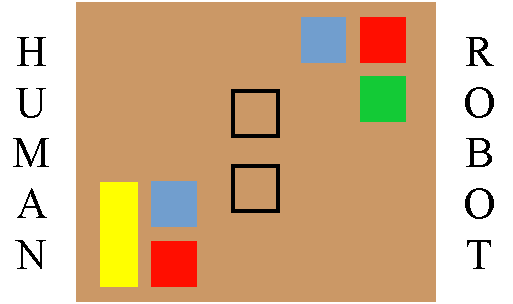
\includegraphics[scale=0.18]{figures/chapter2/task_setup_mini.pdf}}   
	\fancyhead[RO]{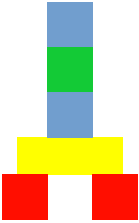
\includegraphics[scale=0.20]{figures/chapter2/task_goal.pdf}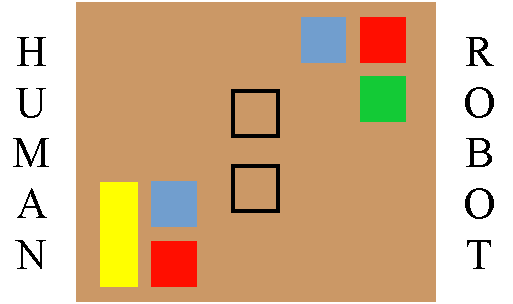
\includegraphics[scale=0.18]{figures/chapter2/task_setup_mini.pdf}\bfseries\thepage}  
	\fancyhead[RE]{\bfseries\nouppercase{\leftmark}}      % Chapter in the right on even pages
	\fancyhead[LO]{\bfseries\nouppercase{\rightmark}}     % Section in the left on odd pages
}%

\usepackage{pdfpages}
\usepackage{makecell}
\usepackage{pdflscape} 
\usepackage{mathtools}
\usepackage[section]{placeins}
\usepackage{afterpage}

%%%%%%%% my commands
\newcommand{\etal}{\textit{et al}.}
\newcommand{\ie}{\textit{i.e.}, }
\newcommand{\eg}{\textit{e.g.}, }
\newcommand{\fact}[3]{\mbox{\textit{#1}(#2, #3)}}
\newcommand{\circledtext}[1]{\raisebox{.5pt}{\textcircled{\raisebox{-.9pt} {#1}}}}
\newcommand{\sparql}{\textsc{SPARQL}}

\newcommand{\algConst}[1]{${\scriptscriptstyle #1}$}
\newcommand{\algNormTextSub}[2]{$\text{#1}_{#2}$}

\newcommand{\aslnumber}[1]{$#1$}
\newcommand{\aslstring}[1]{\textsf{#1}}
\newcommand{\aslvar}[1]{\textcolor{purple}{\textit{#1}}}
\newcommand{\asllabel}[1]{\textbf{#1}}
\newcommand{\annotation}[1]{{\footnotesize #1}}
\newcommand{\rulebody}[1]{\mbox{\hspace{.05\linewidth}}\begin{minipage}[t]{0.9\linewidth}#1.\end{minipage}}
\newcommand{\context}[1]{\begin{minipage}[t]{0.9\linewidth}#1\end{minipage}}
\newcommand{\planbody}[1]{\begin{minipage}[t]{0.9\linewidth}#1.\end{minipage}}
\newcommand{\Jason}[0]{\textbf{\textit{Jason}}}
\newcommand{\sn}{\mbox{\large\textbf{\texttt{\textasciitilde}}}}


\sloppy
\begin{document}
	\setcounter{chapter}{2} %% Numéro du chapitre précédent ;)
	\dominitoc
	\faketableofcontents
	\fi

\chapter{Architectures for Collaborative Robots, Decision and Execution}\label{chapter:chap3}
\chaptermark{Architectures for Decision and Execution}
\minitoc
Robots are machine which need to perceive, decide and act. There are multiple ways to endow a robot with such abilities, with different levels of complexity. When a robot has a complex and generic software architecture, based on models which might be inspired from other fields like psychology, philosophy, neurology, it is referred to as cognitive robot or autonomous robots or intelligent robot...We are interested in such architectures but designed to be implemented in collaborative robots. And, we take an interest in a particular function of these architecture: the decision-making, the supervision of the task, of the interaction.

\section{Existing Architectures for Collaborative Robots}\label{chap3:sec:archi}
``An integrated cognitive architecture can be defined as a single system that is capable of producing all aspects of behaviour, while remaining constant across various domains and knowledge bases''~\cite[p.~104]{chong_2007_integrated}. Kotseruba and Tsotsos reviewed cognitive architectures starting 40 years ago until nowadays. They accounted around three hundred of them and chose to focus their review on 84~\cite{kotseruba_2020_40}. However, the term \emph{cognitive architecture} often refers to an architecture modeling human cognition~\cite{howes_1997_role} and what interest us is to endow robots with cognitive and interactive abilities, not always basing ourselves on human cognition.  

Some cognitive architectures such as ACT-R has been adapted for human-robot interaction (ACT-R/E)~\cite{trafton_2013_act}. The architecture aims at simulating how humans think, perceive and act in the world, strongly based on theory of mind. It is interesting but to understand humans is not enough to make the robot a good collaborators for them, as it lacks abilities concerning the human-aware task and action execution. 

A very complete architecture, CRAM, dealing with problems such as manipulation, perception, plans or beliefs management has been developed by Beetz \etal~\cite{beetz_2010_cram}. However, this architecture is more designed for a robot acting alone than a robot acting in collaboration with a human.

The work of Scheutz and colleagues is compelling, as they proposed a generic architecture, DIARC, for cognitive robots collaborating with humans~\cite{scheutz_2006_utility,scheutz_2019_overview}. In this context, it handles perception, dialogue and different kind of actions. But, the architecture lacks real modeling and awareness of the human at each level.

Rossi \etal{} presented in \cite{rossi_2013_extensible} an architecture to handle multi-modal interaction. In their system, users are able to express their instructions as combinations of different modalities considering that redundancy can be useful. The system is build upon a multi-layered late fusion approach, based on classification. In addition, the system is designed in a way to be easily extensible and easy to modify (\eg possibility to add or remove a modality, possibility to change the classification strategies). The system has been used for example to handle pick-place-carry tasks interacting with a robot through gestures and speech. However, this is for robots following human orders only, and not handling planning and plan execution.

Another architecture worth to be mentioned is the DAC-h3 architecture by Moulin-Frier, Fischer \etal, inspired from biology~\cite{moulin_2017_dac}. It is designed for a robot maintaining social interactions with humans, able to tell narratives and to acquire knowledge thanks to its interactions with humans. As it is mainly dedicated to knowledge acquisition and expression, it lacks planning and execution abilities.

As part of the Platform-Independent Cooperative Human Robot Interaction System, Lallee \etal{} proposed an original architecture for learning and executing shared plans~\cite{lallee_2012_towards}. They developed a way to encode actions in terms of perceptual changes based on motor primitives descriptions. That way, the robot is able to learn new actions as perceptions. Their actions can take several arguments (\eg AGENT put the OBJECT on the RECIPIENT) which enables the system to react and generalize when faced to a new context. The system takes as inputs spoken language interaction and visual perception. It is very interesting but focuses on robots learning objects, actions and plans and not really on collaborative tasks handling. 

Finally, there is the architecture developed and implemented by Lemaignan and colleagues for collaborative robots. All deliberative components of the architecture are human-aware~\cite{lemaignan_2017_artificial}, \ie all of components except the sensorimotor layer. By human-aware components we mean components explicitly taking humans into account, \ie its actions, preferences, abilities, and this based on social norms and models. This architecture is based on the philosophical BDI model developed by Bratman~\cite{bratman_1987_intention,bratman_1988_plans}. It has 3 main concepts defined as the following in computer science:
\begin{bulletList}
	\item \emph{Beliefs}: They are a representation of the agent’s knowledge about the world. ``[They] can be viewed as the informative component of system state''~\cite[p.~313]{rao_1995_bdi}. It is not the word ``knowledge'' that has been chosen to define this concept because what the agent perceives of the environment is in fact the likely state of the environment. There is no certainty, its sensors are not accurate or could malfunction. This way of distinguish knowledge and beliefs is one that can be found in the literature of distributed computing~\cite{lamarre_1994_knowledge}.
	\item \emph{Desires}\footnote{In one of the first implementation, PRS, ``Goals'' notion was used instead of ``Desires''~\cite{georgeff_1989_decision}, then they use it in a interchangeable way in~\cite{georgeff_1991_modeling} and finally choose ``Desires''~\cite{rao_1995_bdi} with the definition given in the AI literature, \eg desires can be many at any instant and may be mutually incompatible. Therefore, a goal will be a chosen desire~\cite{cohen_1990_intention} and concurrent goals are consistent.}: They are a representation of the motivational state of the system. They provide ``information about the objectives to be accomplished or, more generally, what priorities or payoffs are associated with the various current objectives''~\cite{rao_1995_bdi}. 
	\item \emph{Intentions}: They are a representation of the currently chosen course of action (plan). It is the deliberative component of the system. The selected course(s) of action are determined with a deliberative function, according to the beliefs and desires~\cite{rao_1995_bdi}.
\end{bulletList}



\section{The updated LAAS Architecture -- DACOBOT}\label{chap3:sec:rob_archi}

In this section, we present an overview of the robotic architecture, \acrfull{dacobot}, that we collaboratively developed with Guillaume Sarthou and Guilhem Buisan. This architecture model, shown in Figure~\ref{chap3:fig:archi}, has been inspired by the architecture developed by Lemaignan and colleagues~\cite{lemaignan_2017_artificial}, mentioned in the previous section. These architectures are descendant of one of the first architectures for autonomous robots, developed by Alami \etal{}~\cite{alami_1998_architecture}. They have a common characteristic: they are divided into three levels, the decisional level, the execution level and the functional level. Well, these three levels can be compared to the levels presented in the theoretical framework developed by Pacherie and presented in Section~\ref{chap1:subsubsec:neuro_seg}, which is a strong advantage for a robotic architecture dedicated to \acrshort{hri}.

\subsection{Specificities}

All the architectures presented in Section~\ref{chap3:sec:archi} are very interesting but we decided to focus on the last one presented, developed by Lemaignan \etal{}. It seemed relevant to us to pursue this work started in our lab by expanding the components features and refining, consolidating the interactions between these components. The component names and functions of both architectures are the same but most of the implementations are all new and the way they rely on, interact with each other, is as well. All the components of the \acrshort{dacobot} are designed to be human-aware, making the global system human-aware, which is quite rare.

With this architecture, we focus on a given type of \acrlong{hri}: collaborative tasks, joint actions. In this context, the human and the robot share a common space and exchange information through multiple modalities (speech, gesture, gaze). The robot should be able to act on its environment, by manipulating objects and navigate among humans. This function is assured by the Motion Planners and Excutors presented in Section~\ref{chap3:subsubsec:motion}. In order to be aware of its environment, the robot needs perception modalities which are handled by the sensorimotor layer, it can be cameras, lasers, motion capture, force sensors, etc. To avoid each component having to process the data itself in order to be able to use them, the Situation Assessment, presented in Section~\ref{chap3:subsubsec:sa} converts them from geometric data to symbolic data. Moreover, it endows the robot's visual perspective-taking (see Section~\ref{chap1:sec:tom}). Then, these data are stored in \acrlong{kb}s which are introduced in Section~\ref{chap3:subsubsec:kb}, one for the robot and another for the human. Finally, the heart of the architecture, the decision-making process is located in the Supervisor which is the focus of Chapters~\ref{chapter:chap5} and~\ref{chapter:chap6}. In order to make its decisions, the Supervisor relies on the \acrshort{kb}s, the communication through the \acrfull{nlp} and especially the Task Planners presented in Section~\ref{chap3:subsubsec:task_planner}. Once the decision made, it controls the robot through the Motion Planners and Executors and the \acrshort{nlp}. All communication between the components goes through ROS~\cite{quigley_2009_ros}.

\begin{figure}[!ht]
	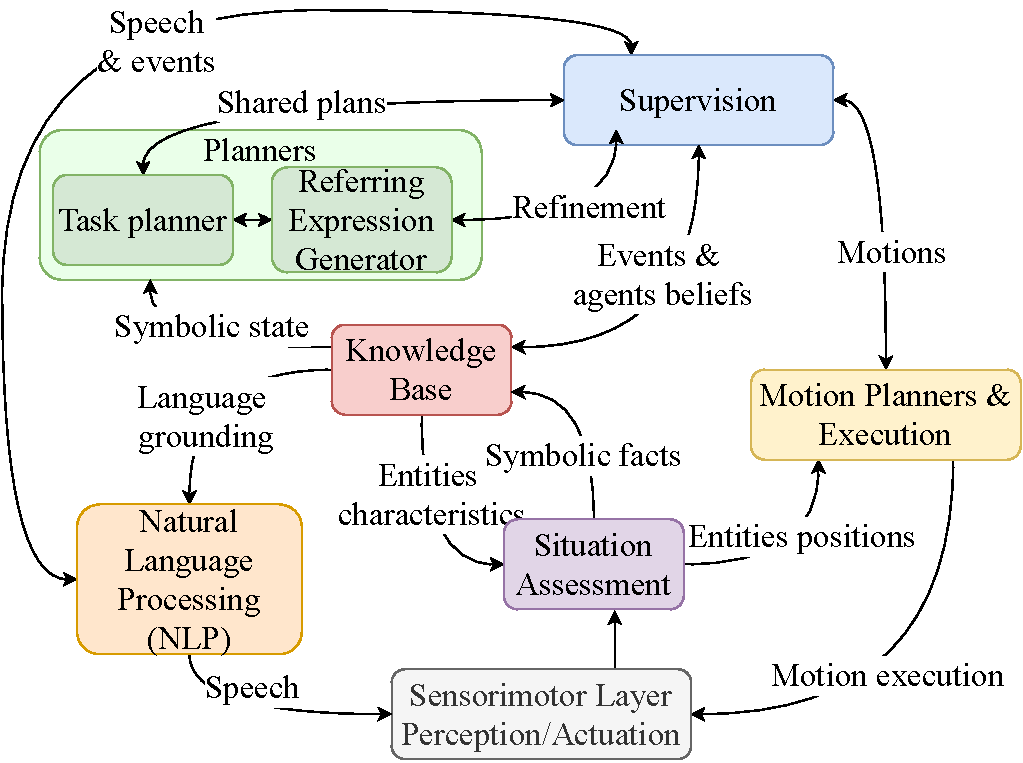
\includegraphics[width=\linewidth]{figures/chapter2/archi_overview.pdf}
	\caption{Overview of the \acrfull{dacobot}.}
	\label{chap3:fig:archi}
\end{figure}

\newpage

\subsection{Architecture components}

\subsubsection{Situation Assessment}\label{chap3:subsubsec:sa}
The Situation Assessment has two roles:
\begin{enumerate}
	\item  to gather different perceptual information and build a geometric representation of the world (\ie elements have associated 3D coordinates), composed of objects and agents; the module runs reasoning processes to interpret this geometric world into a symbolic world, grounding \emph{symbolic facts} which specify object properties, relations between the objects, and relations between the involved agents and the objects. Such component can be implemented with framework like Toaster~\cite{milliez_2014_framework} or Underworld~\cite{lemaignan_2018_underworlds}.
	\item estimate the human's perspective and build an estimation of their world representation; it is the first step allowing to implement the theory of mind principles (see Section~\ref{chap1:sec:tom}).
\end{enumerate}

Thus, the Situation Assessment represents the state of the world like it is perceived by the agents, the human and the robot. It is in the form of symbolic facts, such as \fact{isOnTopOf}{cube\_1}{cube\_3} or \fact{isReachableBy}{cube\_2}{human\_0}. The first element of this triplet is called the property, the second one is the subject and the last one is the object.

\subsubsection{Knowledge Bases}\label{chap3:subsubsec:kb}

Knowledge management is central in a robotic architecture. As this architecture is specific to \acrshort{hri}, the knowledge handling should be as well. Indeed, during an interaction, belief divergences may arise between agents and thus how this should be represented? Each agent, human and robot, should have their own knowledge base. Software developed by Guillaume Sarthou with whom we collaborated closely allow this. They are two of them: Ontologenius\footnote{\url{https://github.com/sarthou/ontologenius}}~\cite{sarthou_2019_ontologenius} for the semantic knowledge and Mementar\footnote{\url{https://github.com/sarthou/mementar}} for the episodic one. They are fully adapted to \acrshort{hri} applications by representing the robot's knowledge and the estimation of the partners' knowledge separately, which refers to the psychological concept of the ``self-other distinction'' as coined in joint action studies~\cite{pacherie_2012_agency}.  

\paragraph{Semantic knowledge base} stores common-sense knowledge based on three concepts, in the form of an ontology\footnote{An ontology is a way to represent knowledge}: (1) classes representing the possible types of entities known by the agent (\eg Cube is a class inheriting from the class Pickable), (2) properties which can denote both the attributes of objects (\eg the color) and the relations between the objects (\eg which object is on which other one), and (3) object instantiations also called individuals (\eg cube\_3 is an object present in the environment, of the class Cube).

It is in charge of representing the environment elements meaning, the objects' and agents' types (\eg a cube is an object), their applicable properties (\eg cube\_1 has color blue), the descriptions and parameters of the actions, a part of the language model with verbs or pronouns, and their names in natural language.
	
Besides, it is also in charge of representing the current symbolic world-state (the computed facts, \eg \fact{isOnTof}{cube\_2}{table\_1}) and thus the instantiation of the concepts in terms of physical (\eg this particular block) or abstract (\eg this particular action instance) entities. Moreover, it reasons on it, making deductions and links between facts, creating new ones (\eg after receiving \fact{isOnTof}{cube\_2}{table\_1} and it computes \fact{isUnder}{table\_1}{cube\_2}). Finally, it stores knowledge about activities grounded in space and time (\eg object\_1245 has been put on the table\_2 by robot (action ID 475)).

To access to the knowledge stored in Ontologenius, the Supervisor can make a request to know if a given fact exists or ask an information about a class, a property or an object instantiation (\eg the Supervisor can ask the human understandable name of pick\_action which is ``pick''). Another way is to subscribe to updates (addition or deletion) for given facts (\ie facts necessary to the task or the Supervisor functioning). It is useful for keeping updates about the environment and avoid to be snowed under too much data. For example, the Supervisor can ask to receive every update (addition or deletion) of any fact belonging to the type \fact{isOnTopOf}{Cube}{Table}. In this case, it will receive the addition of \fact{isOnTopOf}{cube\_2}{table\_1} but not of \fact{isOnTopOf}{spoon}{table\_1}. It is possible to either specify the class or individual of the subjects/objects that should be concerned by the subscription, or to receive every facts (\eg it can subscribe to receive additions of the human looking at the robot |[add]human_0$\lvert$isLookingAt$\lvert$robot| or to receive all updates about every objects that the human looks at |[?]human_0$\lvert$isLookingAt$\lvert$?|). The way the Supervisor chooses which fact it should receive is described in Chapter~\ref{chapter:chap6}.

\paragraph{Episodic knowledge base} is represented as a timeline, keeping track of the symbolic facts computed over time (\eg action ID 475 started at 3286 seconds and was over at 3290 seconds), either by the Situation Assessment, the Semantic Knowledge Base or the Supervisor. One of the possible use is to refer to past actions when communicating with the human~\cite{sarthou_2021_extending}.


\subsubsection{Human-Aware Motion Planners and Execution}\label{chap3:subsubsec:motion}
The motion planners allow the robot to execute human-aware motion actions. According to the task needs, several planners might be involved for a same task. Indeed, in a task requiring object manipulation, the robot will need a motion planner able to plan for pick, place and drop actions, such as MoveIt\footnote{\url{https://moveit.ros.org/}} or GTP which is human-aware~\cite{waldhart_2016_novel}, and a home-made software handling the execution these trajectories\footnote{\url{https://github.com/YannickRiou/pr2_mtc}}. Moreover, in collaborative tasks, an agent might be led to hand over an object to their partner, in this case could be used a dedicated planner~\cite{mainprice_2012_sharing}. Finally, the robot might need to move in the environment, but when moving in a environment with humans, it should navigate being aware of them for safety and legibility. Thus, the robotic architecture should integrate co-navigation planner and executor such as HATEB-2~\cite{singamaneni_2020_hateb}. 

These planners produce trajectories and moves on request of the Supervisor. During execution, they send feedbacks and results about the state execution, in this way the Supervisor can receive data about errors, unexpected events or the estimated remaining time of execution. It allows the Supervisor, then, to decide and act based on this information.

\subsubsection{Human-Aware Task Planner}\label{chap3:subsubsec:task_planner}
We can distinguish two situations in which a collaborative robot needs a human-aware task planner: 
\begin{inlineEnumerate}
	\item when it performs a task on its own but a human is nearby and so it should consider potential conflicting actions with them, and
	\item when it performs a task with a human.
\end{inlineEnumerate} 
In the first situation, it might consider asking the human's help whereas in the second one it needs to plan for both agents' actions. 

The human-aware task planners generate symbolic shared plans in which each agent, human and robot, has actions of the task assigned to them, depending on criteria such as programmer-defined costs, minimization of the human's effort, and their preferences and comfort. Such plans are constructed to be as respectful as possible of social constraints which benefits to the also human-aware Supervisor. However, the human is neither an agent that the planner can directly control or an agent that will know the complete plan. Thus, it allows the robot to plan by emulating the human decision, action, and reaction processes. 

We worked with two human-aware task planners: \acrfull{hatp}~\cite{lallement_2014_hatp}, and a recent and prototypical planner called \acrfull{hatpehda}~\cite{buisan_2021_human}.

The \acrfull{hatp} proposes a hierarchical approach to multi agents task planning. This \acrfull{htn}-based planner is able to elaborate a multi agents plan based on a single \acrshort{htn} tree. \acrshort{htn} planning aims at decomposing abstract tasks into primitive tasks by choosing from a list of available context-dependent refinements for each abstract task, ensuring that preconditions and effects of refined primitives tasks are satisfied throughout the created plan. This formalism is suitable for human-robot interactions as it allows the robot to communicate about the plan more easily. \acrshort{hatp} has been specially designed to integrate a number of features that are meant to promote the synthesis of plans that are acceptable by humans and easily if not trivially understandable by them. It allows to specify the humans and robot capabilities in terms of actions they can execute. Several aspects such as human preferences and comfort, estimation of human effort to achieve a task in a given context and ``social rules'' are used in a cost-based approach to build ``sufficiently good'' human-robot shared plans.

The \acrfull{hatpehda} also proposes a hierarchical approach to multi agents task planning. This approach relies on a representation of each agent considered by the planner, with their own beliefs, agenda, stream of execution and action model. The action models are represented as \acrshort{htn}s which are explored consecutively yet differently if the agent is controllable (robots) or uncontrollable but rational (humans). We highlight two main advantages over \acrshort{hatp}. The first one is the computation of conditional plans, allowing to anticipate situations where the human may perform multiple different actions equally making the plan progressing, or may decide to act or wait for the robot to act. Then, the decision of which branch of the plan to follow is postponed at execution time and handled by the Supervisor. Another advantage is to explicitly represent robot to human communication needs for beliefs alignment, goal sharing or action requests. Indeed, \acrshort{hatp} generates plans in which it is unknown what needs to be communicated to the human or what can be easily guessed (\ie which is predictable) by the human. Finally, like in \acrshort{hatp}, it is possible to define ``social costs functions''. By doing so, the planner can penalize non-acceptable sequence of robot actions (\eg serving a meal just after taking out the trash) or non-satisfactory human required contribution (\eg or requesting the human to perform small tasks multiple times instead of giving the big picture of the real task to perform).


\subsubsection{Supervision}
The Supervision is the puppet master of the system, embedding the robot high-level decisions, controlling its behavior and trying to react to contingencies, always considering the human it is interacting with. It is not standalone, relying on the components described above to be able to take decisions, be aware of the environment and make the robot moves. It will be the subject of Chapters~\ref{chapter:chap5} and~\ref{chapter:chap6}.

\newpage

\section{Conclusion}

In the context of this thesis, it was important to present the robotic architecture in which the supervisor is integrated. Indeed, it cannot run the robot by itself, it needs the features offered by the other components but not whatever planner or navigation for example. It relies on human-aware ones. 

We presented an overview of existing robotic architectures, with some of them dedicated to human-robot collaboration. We chose to carry on the development of the robotic architecture designed by our research team a few years ago. The new architecture we conceived has the same component blocks than the one of Lemaignan \etal{}, however all our components are different and we refined and reinforced the links between the components, especially with the \acrlong{kb}. 

We introduce the components of the architecture: the Situation Assessment, the \acrshort{kb}s, the Human-aware Motion Planners and Executors, the Human-aware Task Planners and the Supervision. We voluntarily left aside the \acrshort{nlp} and the perception as no one in our research team work one these subjects. We use freeware or open-source software to perform our experiments. As we can see, our architecture is quite sophisticated which makes the supervisor essential to manage all these components during an interaction. After giving the global picture of the system, we will focus on the supervisor in the next chapters.

\ifdefined\included
\else
\bibliographystyle{acm}
\bibliography{These}
\end{document}
\fi